\begin{figure*}[t]
	\centering
	\addtolength{\tabcolsep}{-4.5pt}
	\begin{tabular}{ccccccccc}
		photo & sample-1 & sample-2 & sample-3 & & photo & sample-1 & sample-2 & sample-3
		\\
		\begin{overpic}[width=\resultwidth]{images/real/bump3/out/target.png}
			\imglabel{Bump-3}
		\end{overpic} &
		\includegraphics[width=\resultwidth]{images/real/bump3/out/good1.png} &
		\includegraphics[width=\resultwidth]{images/real/bump3/out/good2.png} &
		\includegraphics[width=\resultwidth]{images/real/bump3/out/bad1.png} &
		&
		\begin{overpic}[width=\resultwidth]{images/real/bump2/out/target.png}
			\imglabel{Bump-4}
		\end{overpic} &
		\includegraphics[width=\resultwidth]{images/real/bump2/out/good1.png} &
		\includegraphics[width=\resultwidth]{images/real/bump2/out/good2.png} &
		\includegraphics[width=\resultwidth]{images/real/bump2/out/bad1.png}
		\\
		\begin{overpic}[width=\resultwidth]{images/real/leather/out/target.jpg}
			\imglabel{Leather-3}
		\end{overpic} &
		\includegraphics[width=\resultwidth]{images/real/leather/out/good1.jpg} &
		\includegraphics[width=\resultwidth]{images/real/leather/out/good2.jpg} &
		\includegraphics[width=\resultwidth]{images/real/leather/out/bad1.jpg} &
		&
		\begin{overpic}[width=\resultwidth]{images/real/leather2/out/target.png}
			\imglabel{Leather-4}
		\end{overpic} &
		\includegraphics[width=\resultwidth]{images/real/leather2/out/good1.png} &
		\includegraphics[width=\resultwidth]{images/real/leather2/out/good2.png} &
		\includegraphics[width=\resultwidth]{images/real/leather2/out/bad1.png}
		\\
		\begin{overpic}[width=\resultwidth]{images/real/leather3/out/target.png}
			\imglabel{Leather-5}
		\end{overpic} &
		\includegraphics[width=\resultwidth]{images/real/leather3/out/good1.png} &
		\includegraphics[width=\resultwidth]{images/real/leather3/out/good2.png} &
		\includegraphics[width=\resultwidth]{images/real/leather3/out/bad1.png} &
		&
		\begin{overpic}[width=\resultwidth]{images/real/leather4/out/target.png}
			\imglabel{Leather-6}
		\end{overpic} &
		\includegraphics[width=\resultwidth]{images/real/leather4/out/good1.png} &
		\includegraphics[width=\resultwidth]{images/real/leather4/out/good2.png} &
		\includegraphics[width=\resultwidth]{images/real/leather4/out/bad1.png}
		\\
		\begin{overpic}[width=\resultwidth]{images/real/plaster/out/target.jpg}
			\imglabel{Plaster-3}
		\end{overpic} &
		\includegraphics[width=\resultwidth]{images/real/plaster/out/good1.jpg} &
		\includegraphics[width=\resultwidth]{images/real/plaster/out/good2.jpg} &
		\includegraphics[width=\resultwidth]{images/real/plaster/out/bad1.jpg} &
		&
		\begin{overpic}[width=\resultwidth]{images/real/plaster2/out/target.png}
			\imglabel{Plaster-4}
		\end{overpic} &
		\includegraphics[width=\resultwidth]{images/real/plaster2/out/good1.png} &
		\includegraphics[width=\resultwidth]{images/real/plaster2/out/good2.png} &
		\includegraphics[width=\resultwidth]{images/real/plaster2/out/bad1.png}
		\\
		\begin{overpic}[width=\resultwidth]{images/real/flake/out/target.jpg}
			\imglabel{Metallicflake-3}
		\end{overpic} &
		\includegraphics[width=\resultwidth]{images/real/flake/out/good1.jpg} &
		\includegraphics[width=\resultwidth]{images/real/flake/out/good2.jpg} &
		\includegraphics[width=\resultwidth]{images/real/flake/out/bad1.jpg} &
		&
		\begin{overpic}[width=\resultwidth]{images/real/flake2/out/target.png}
			\imglabel{Metallicflake-4}
		\end{overpic} &
		\includegraphics[width=\resultwidth]{images/real/flake2/out/good1.png} &
		\includegraphics[width=\resultwidth]{images/real/flake2/out/good2.png} &
		\includegraphics[width=\resultwidth]{images/real/flake2/out/bad1.png}
		\\
		\begin{overpic}[width=\resultwidth]{images/real/metal/out/target.png}
			\imglabel{Brushmetal-3}
		\end{overpic} &
		\includegraphics[width=\resultwidth]{images/real/metal/out/good1.png} &
		\includegraphics[width=\resultwidth]{images/real/metal/out/good2.png} &
		\includegraphics[width=\resultwidth]{images/real/metal/out/bad1.png} &
		&
		\begin{overpic}[width=\resultwidth]{images/real/wood/out/target.jpg}
			\imglabel{Wood-3}
		\end{overpic} &
		\includegraphics[width=\resultwidth]{images/real/wood/out/good1.jpg} &
		\includegraphics[width=\resultwidth]{images/real/wood/out/good2.jpg} &
		\includegraphics[width=\resultwidth]{images/real/wood/out/bad1.jpg}
		\\
		\begin{overpic}[width=\resultwidth]{images/real/wood2/out/target.png}
			\imglabel{Wood-4}
		\end{overpic} &
		\includegraphics[width=\resultwidth]{images/real/wood2/out/good1.png} &
		\includegraphics[width=\resultwidth]{images/real/wood2/out/good2.png} &
		\includegraphics[width=\resultwidth]{images/real/wood2/out/bad1.png} &
		&
		\begin{overpic}[width=\resultwidth]{images/real/wood3/out/target.png}
			\imglabel{Wood-5}
		\end{overpic} &
		\includegraphics[width=\resultwidth]{images/real/wood3/out/good1.png} &
		\includegraphics[width=\resultwidth]{images/real/wood3/out/good2.png} &
		\includegraphics[width=\resultwidth]{images/real/wood3/out/bad1.png}
	\end{tabular}
	\caption{\label{fig:real}
		Results of our MCMC sampling on \textbf{real} inputs. For each example, the first column is the real target image (photo). We show MCMC samples in the other columns, where sample-1 and sample-2 are chosen closer to the peak of the posterior distribution, and sample-3 is further away. Note that the target images for Plaster-4 and Wood-5 are captured under natural illumination, while the corresponding synthetic images still assume collocated flash illumination; despite this mismatch, the estimated material parameters are still reasonable. Note, target images for Leather-4, Leather-6 and Wood-4 are from the publicly released dataset of \cite{Aittala2016}. For more results please refer to supplemental materials.
	}
\end{figure*}
